\section{Experimental Setup Details}
\label{app:experimental_setup}

\subsection{Data Construction and Split}
\label{app:data_construction}

\paragraph{Persona Collection.}
We collect a diverse set of 2{,}100 character persona profiles spanning multiple domains, including game characters, film and television characters, and real-world figures, split into a 2{,}000-persona training set and a 100-persona held-out test set. As illustrated in Fig.~\ref{fig:persona_distribution}, the test personas cover five major categories: Fictional (43\%), Celebrities (29\%), Social (14\%), Creatures (9\%), and Others (5\%), demonstrating that our evaluation is domain-agnostic and generalizable across diverse character types.

\begin{figure}[t]
  \centering
  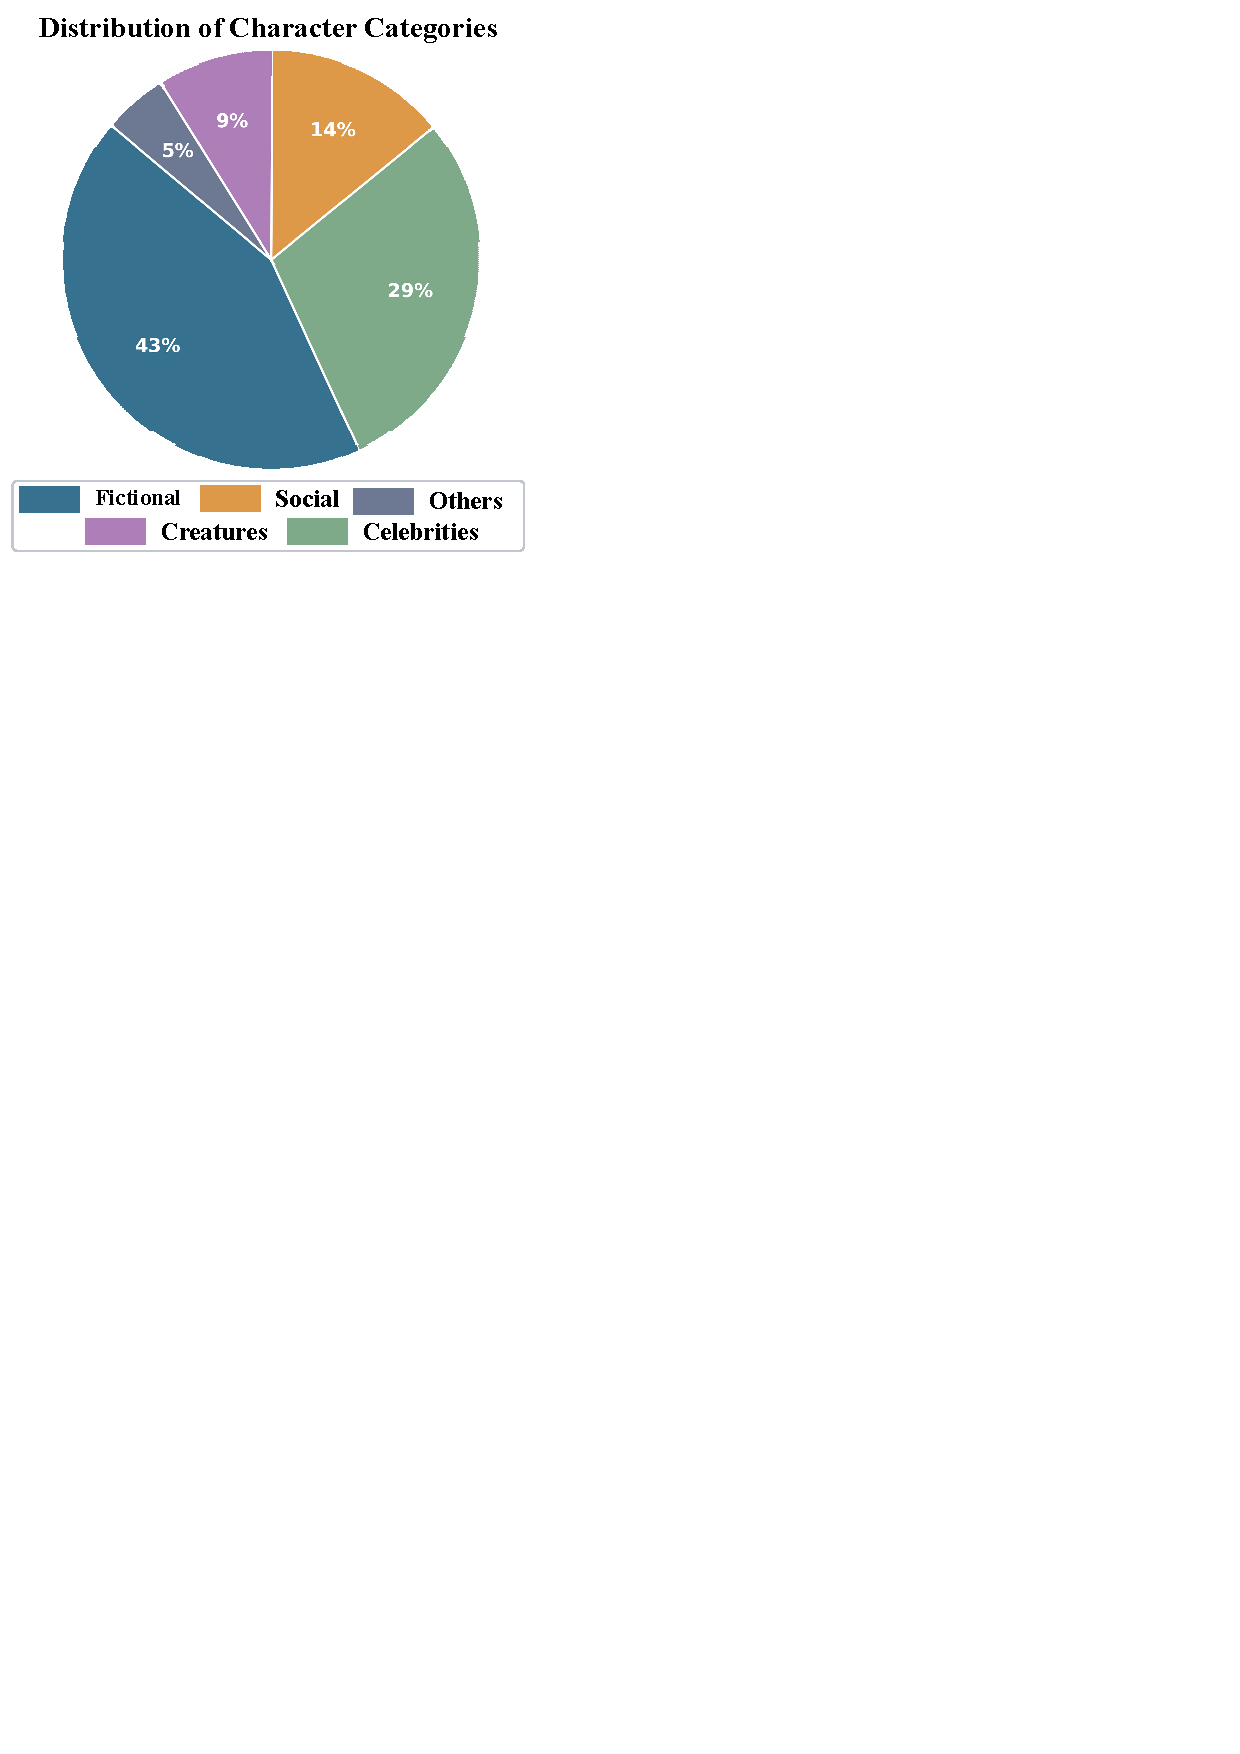
\includegraphics[width=\columnwidth, trim = 0 20cm 11.8cm 0, clip]{latex/Image/appendix-persona-pie-0520.pdf}

  \caption{Distribution of character categories in the test persona set.}
  \label{fig:persona_distribution}
\end{figure}


\paragraph{SFT Data Construction.}
For supervised fine-tuning, we construct one 50-turn trajectory for each of the 2{,}000 training personas using the multi-turn lookahead search in Section~\ref{sec:stage1}. The search uses a segment length of $T=10$ turns and $K=5$ sequential steps. At each step, $N_s=2$ candidate character agents are sampled from a global pool of $N=5$ models (Gemini-3-Pro, Claude Sonnet 4.6, GPT-5.4, Qwen-Plus-Character, and Doubao-1.5-Pro-Character). Both candidates continue from the same committed prefix and interact with the Doubao-1.5-Pro-Character user simulator for 10 turns. The higher-scoring segment is appended to the committed trajectory. The resulting 2{,}000 reward-optimized trajectories are used for SFT.

% For supervised fine-tuning, we construct a 50-turn dialogue trajectory for each of the 2{,}000 training personas using the Reward-Driven Trajectory Construction via Multi-turn Lookahead Search procedure described in Section~\ref{sec:train}. Specifically, with a chunk size of $T=10$ turns, the process advances in 5 steps. At each step, 2 candidate character agents are sampled from a diverse pool of 5 (Gemini-3-pro, Claude Sonnet 4.6, GPT-5.4, Qwen-plus-character, and Doubao-1.5-pro-character) to perform chunk-level rollouts. Each candidate interacts with the user simulator (Doubao-1.5-pro-character) for 10 turns, and the chunk yielding the highest session-level evaluation score is selected and appended to the confirmed trajectory. This produces high-quality, reward-optimized 50-turn trajectories that serve as the SFT training data. The detailed prompt templates are provided in Appendix~\ref{app:prompt}.

\paragraph{DSPO Preference Data.}
For DSPO, each of the 2{,}000 training personas yields five raw winner--loser comparisons, producing 10{,}000 raw segment-level preference pairs. To reduce position bias in LLM-based judgments, we evaluate every pair in both presentation orders, $(A,B)$ and $(B,A)$, and retain the pair only when the preferred segment is consistent across both orders. This bidirectional consistency filter retains 6{,}089 preference pairs for DSPO training.

% For the DSPO stage, we reuse the same 2{,}000 training personas. The preference pairs are directly obtained from the lookahead search process described in Section~\ref{sec:stage1}: at each step, the winner and loser segments under the same prefix naturally form a preference pair. In total, we construct 6{,}000 session-level preference pairs.

\paragraph{Test Set.}
The test set consists of 100 persona-context pairs whose personas are entirely disjoint from those used in training. For each test persona, an initial dialogue history $\mathcal{H}_0$ of variable length (0--50 turns) is constructed using the same chunk-based search procedure as in training. During evaluation, each model under test continues the conversation from the given persona and context by interacting with the user simulator for 10 turns, producing the session trajectory to be evaluated.


% \begin{figure}[t]
%   \centering
%   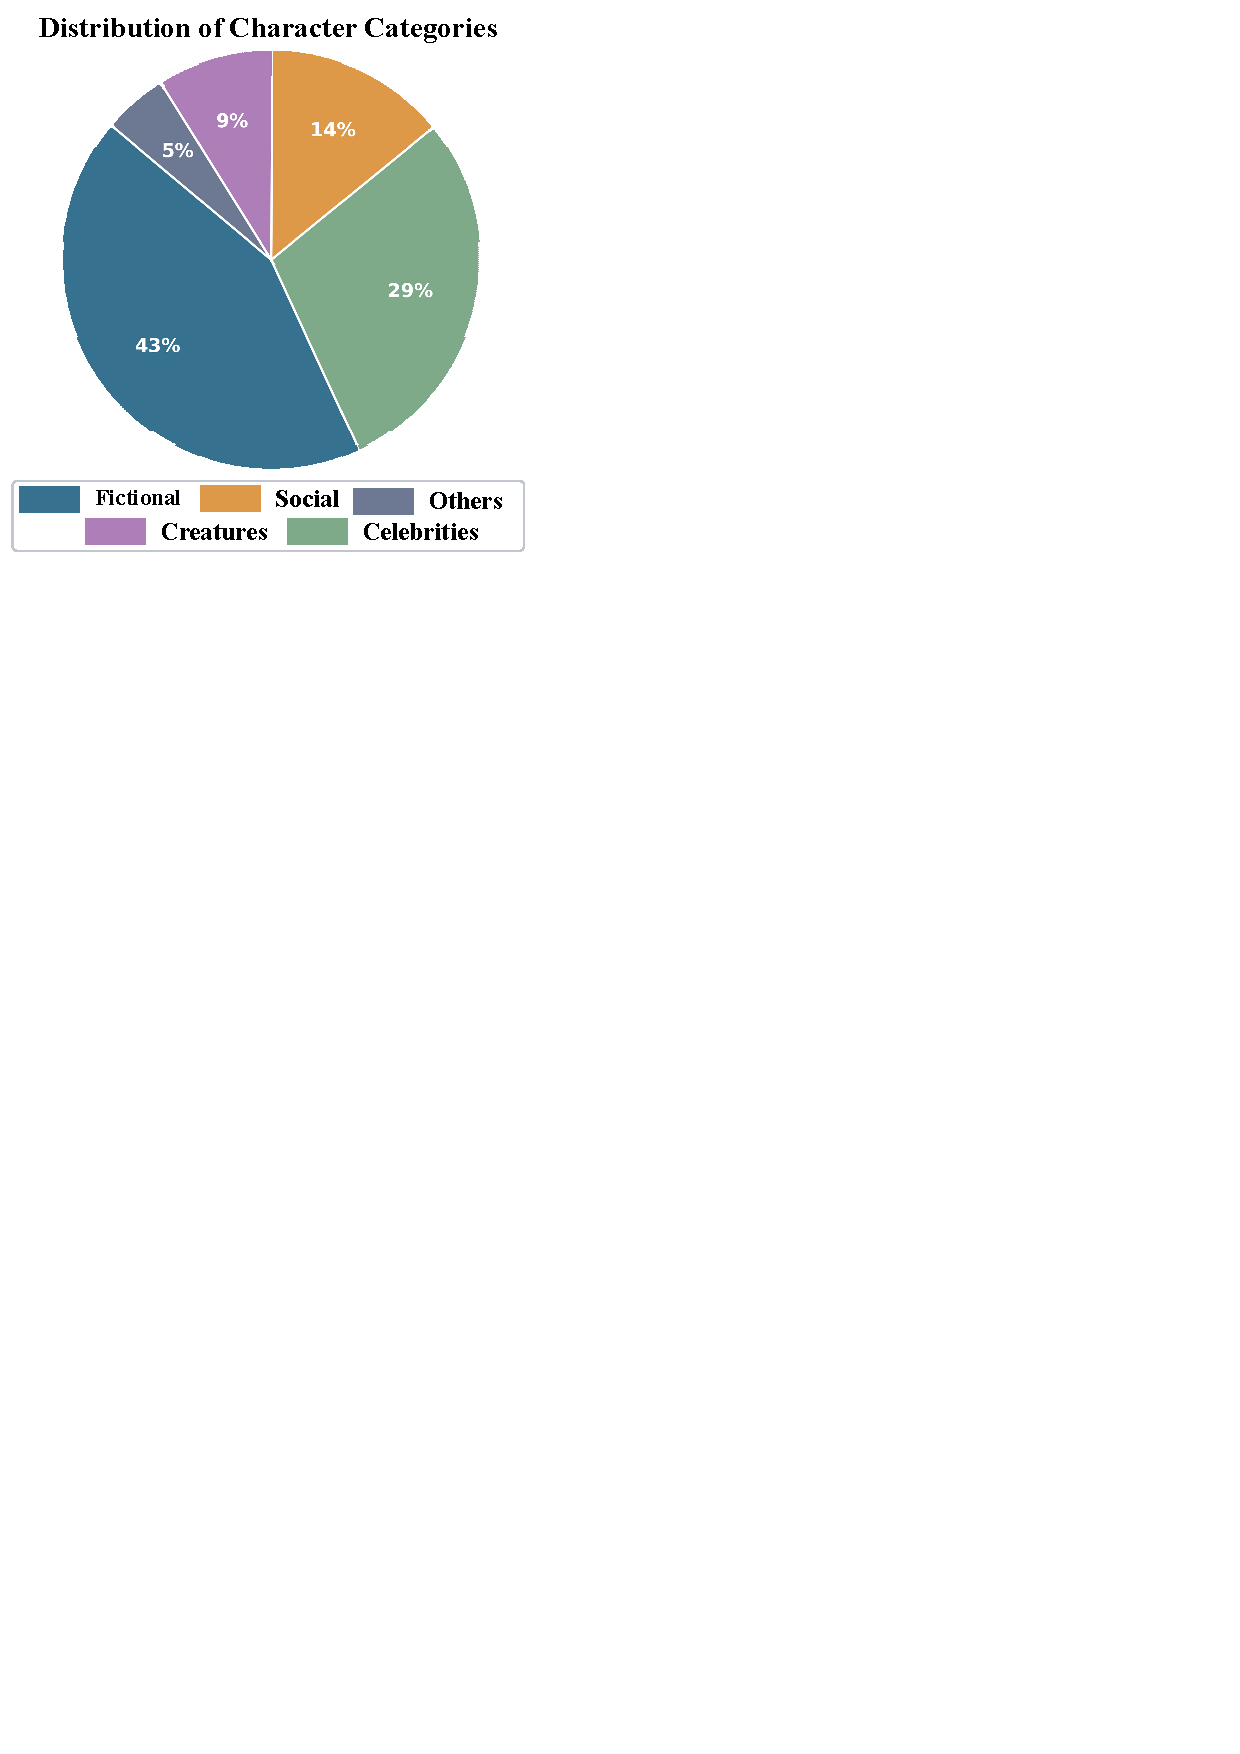
\includegraphics[width=\columnwidth, trim = 0 20cm 11.8cm 0, clip]{latex/Image/appendix-persona-pie-0520.pdf}

%   \caption{Distribution of character categories in the test persona set.}
%   \label{fig:persona_distribution}
% \end{figure}


\paragraph{User Simulator Configuration.}
Throughout all stages (data construction, training, and evaluation), Doubao-1.5-pro-character serves as the user simulator. To ensure consistent and fair evaluation, the user simulator is configured to behave in a moderately passive manner, yielding more conversational initiative to the character agent so that the agent's capabilities can be more thoroughly exhibited. The temperature is set to 1.0. Additionally, the role-playing prompt instructs the simulator to adopt a relatively reactive conversational style, avoiding overly proactive or leading utterances. The complete prompt is provided in Appendix~\ref{app:prompt}.



\subsection{Model Training Details}
\label{subsec:training_details}

We leverage the LLaMA-Factory framework \cite{zheng2024llamafactory} with DeepSpeed ZeRO-3 for the distributed training of DynSess-Character. The training pipeline consists of two stages: (1) Supervised Fine-Tuning (SFT) on the reward-driven trajectories constructed via chunk-based search, and (2) Session-level Policy Optimization using either DSPO (off-policy) or GSRPO (on-policy). Both stages utilize the AdamW optimizer with a warmup ratio of $0.1$.

\paragraph{Supervised Fine-Tuning (SFT).}
The SFT data is formatted in the ShareGPT multi-turn conversation format. We fine-tune the base Qwen3 models (8B and 32B) for 1 epoch with a learning rate of $1 \times 10^{-5}$ and a warmup ratio of 0.1.


\paragraph{Direct Session Preference Optimization (DSPO).}
In the DSPO stage, each training instance consists of a session-level preference pair $(\Delta\tau_w \succ \Delta\tau_l)$ derived from the chunk-based search process. The model is trained for 2 epochs with a learning rate of $1 \times 10^{-6}$, using the reference-regularized pairwise objective defined in Eq.~\ref{eq:dspo}. The KL-divergence coefficient $\beta$ is set to 0.1.

\paragraph{Group Session Relative Policy Optimization (GSRPO).}
In the GSRPO stage, we use the same 2{,}000 training personas. The current policy $\pi_\theta$ interacts with the user simulator on-policy to generate $M=8$ complete sessions per persona. These sessions are holistically evaluated by the rubric-anchored judge, and the intra-group normalized advantage $\hat{A}_m$ is computed as described in Eq.~\ref{advantage}. The policy is then updated using the token-level clipped surrogate objective (Eq.~\ref{grspo}) with $\epsilon = 0.2$. The model is trained for 2 epochs with a learning rate of $1 \times 10^{-6}$.

\paragraph{Hardware.}
The 8B model is trained on 8$\times$ NVIDIA A800 (80\,GB) GPUs, while the 32B model is trained on 8$\times$ NVIDIA H200 (141\,GB) GPUs.


\subsection{Baseline Models and Inference Settings}
\label{app:baseline_models}

% TODO: Add specific model versions, Hugging Face checkpoints, and inference parameters (temperature, top-p, max_tokens) for each baseline.

\paragraph{General-Purpose Models.}
We evaluate GPT-5.4, Gemini-3-pro, Claude Sonnet 4.6, and DeepSeek-V3.2. API-based models are accessed through their official endpoints.

\paragraph{Role-Playing Models.}
We compare against Doubao-1.5-pro-character, Qwen-plus-character, MiniMax-M2-HER (32B), and Coser (70B). API-based models are accessed through their official endpoints; open-weight models are obtained from Hugging Face.

\paragraph{Evaluator Baselines.}
For evaluator comparison (Tab.~\ref{tab:eval-model}), we include CharacterJudge~\citep{zhou2025characterbench}, CharacterRM~\citep{tu-etal-2024-charactereval}, RMTBench~\citep{xiang-etal-2025-rmtbench}, and CharacterArena~\citep{ye-etal-2025-cpo}. For each baseline, we follow the evaluation prompts and judge models specified in the original papers to ensure fair comparison.


\subsection{Evaluation Protocol}
\label{app:evaluation_protocol}

\paragraph{Judge Model.}
We use Gemini-3-Flash as the LLM evaluator $J$ for all \textbf{DynSess-Eval} scoring. The choice of Gemini-3-Flash balances evaluation quality with computational efficiency, enabling large-scale evaluation across multiple models and dimensions.

\paragraph{Scoring Procedure.}
For each model under evaluation, the multi-agent simulation produces a session trajectory $\tau$. Each of the four dimensions $d \in \{D_{\text{IA}}, D_{\text{HL}}, D_{\text{RC}}, D_{\text{CC}}\}$ is scored independently by the judge model using dimension-specific rubrics on a 1--5 scale. To reduce variance from stochastic generation, we evaluate each session trajectory 3 times per dimension and report the average score. The overall session score is computed as the average of the four dimension scores.

\paragraph{Evaluation Dimensions.}
We detail the four session-level evaluation dimensions below. Each dimension is assessed with a dedicated rubric anchored at a baseline score of 3 (pass), with explicit deduction criteria and bonus evidence requirements (see Appendix~\ref{app:prompt} for full prompt templates).

\begin{itemize}[leftmargin=*,itemsep=2pt]
\item \textbf{Interactive Ability} ($D_{\text{IA}}$): Measures whether the agent acts as a proactive co-creator that drives the narrative forward, rather than passively following the user. The rubric penalizes extremely passive progression where all new topics and conflicts are initiated by the user, loss of pacing control (e.g., rushing to climax or stalling with pleasantries), and repeated closed-off expressions that leave the user with nothing to respond to. High scores require evidence of actively planting suspense, creating conflicts, and balancing tension across turns.

\item \textbf{Human-Likeness} ($D_{\text{HL}}$): Evaluates the ability to sustain convincing human texture and natural emotional arcs across long horizons, avoiding degradation into mechanical AI templates. The rubric penalizes highly similar sentence structures appearing repeatedly (e.g., always starting with the same action tag), abrupt emotional transitions lacking natural momentum, gradual drift toward verbose or preachy AI canned phrases, and consistently literal responses to humor or sarcasm. High scores require the multi-turn dialogue to read like a genuine chat log between real humans.

\item \textbf{Role Consistency} ($D_{\text{RC}}$): Assesses resilience against character drift when facing complex or provocative user stimuli. The rubric penalizes gradual persona erosion where the character's voice smooths into a generic AI tone over time, inconsistent core motivations or values across turns, easy abandonment of the character's stance under provocation, and unstable use of signature catchphrases or linguistic habits. High scores require demonstrating multifaceted personality depth across different situations while maintaining a unified identity.

\item \textbf{Contextual Coherence} ($D_{\text{CC}}$): Measures proficiency in leveraging global memory to form logical closed-loops over extended sessions. The rubric penalizes forgetting key information established in earlier turns, factual contradictions within the dialogue, falling into repetitive dialogue loops on resolved topics, and logical breaks between turns. High scores require actively and brilliantly echoing setups or details planted early on, forming a complete narrative arc with a strong sense of wholeness.
\end{itemize}

\paragraph{Prompt Templates.}
The complete prompt templates for the User Agent, Character Agent, and the four dimension-specific evaluation rubrics are provided in Appendix~\ref{app:prompt}.


\subsection{Human Annotation Protocol}
\label{app:human_annotation}

\paragraph{Annotators and Procedure.}
We recruit 3 annotators for the human evaluation. Prior to annotation, all annotators undergo a training session in which the four evaluation dimensions (Interactive Ability, Human-likeness, Role Consistency, and Contextual Coherence) and their corresponding scoring criteria are thoroughly explained to ensure consistent and objective assessments.
For the evaluator validation benchmark (Tab.~\ref{tab:eval-model}), annotators engage in 50-turn conversations with five closed-source role-playing models (Qwen-plus-character, Doubao-1.5-pro-character, GPT-5.4, Gemini-3-pro, and Claude Sonnet 4.6) under 8 different character personas per model, yielding 40 annotated sessions in total. These human scores serve as the ground truth for evaluating automatic evaluators.
For the model comparison (Tab.~\ref{tab:model-performance-human}), each model under comparison interacts with the user simulator for 10 turns on the 100 held-out test personas. The annotators independently score each resulting session trajectory on the four dimensions (1--5 scale), and the final human score for each model is averaged across annotators and test personas.

\begin{table}[t!]
\centering
% \small
\caption{Statistics of different models including Mean, Standard Deviation, Range, and Coefficient of Variation.}
\label{table:stability_analysis}
\resizebox{\columnwidth}{!}{%
\begin{tabular}{lcccc}
\toprule
\textbf{Model} & \textbf{Mean ($\mu$)} & \textbf{Std. Dev ($\sigma$)} & \textbf{Range} & \textbf{CV (\%)} \\
\midrule
Claude Sonnet 4.6 & 4.35 & 0.05 & 0.16 & 1.16 \\
Gemini-3-pro & 4.12 & 0.036 & 0.1 & 0.87 \\
Doubao-1.5-pro-character & 3.96 & 0.058 & 0.15 & 1.45 \\
Coser-70B & 2.87 & 0.064 & 0.16 & 2.2 \\
GPT-5.4 & 4.29 & 0.058 & 0.17 & 1.39 \\
\bottomrule
\end{tabular}%
}
\end{table}

\begin{table*}[t!]
\centering
\caption{Per-dimension stability analysis. We report Std.\ Dev ($\sigma$) and Coefficient of Variation (CV\%) for each model across the four evaluation dimensions. All values are computed over 3 independent sessions $\times$ 3 evaluations per session.}
\label{tab:stability_per_dim}
\resizebox{\textwidth}{!}{%
\begin{tabular}{l cc cc cc cc}
\toprule
\multirow{2}{*}{\textbf{Model}} & \multicolumn{2}{c}{\textbf{Interactive Ability}} & \multicolumn{2}{c}{\textbf{Human-Likeness}} & \multicolumn{2}{c}{\textbf{Role Consistency}} & \multicolumn{2}{c}{\textbf{Contextual Coherence}} \\
\cmidrule(lr){2-3} \cmidrule(lr){4-5} \cmidrule(lr){6-7} \cmidrule(lr){8-9}
& $\sigma$ & CV(\%) & $\sigma$ & CV(\%) & $\sigma$ & CV(\%) & $\sigma$ & CV(\%) \\
\midrule
Claude Sonnet 4.6 & 0.063 & 1.63 & 0.060 & 1.54 & 0.086 & 1.73 & 0.114 & 2.55 \\
Gemini-3-pro & 0.065 & 1.78 & 0.053 & 1.55 & 0.050 & 0.99 & 0.064 & 1.45 \\
Doubao-1.5-pro-character & 0.071 & 1.99 & 0.098 & 2.93 & 0.086 & 1.81 & 0.086 & 2.03 \\
Coser-70B & 0.063 & 2.54 & 0.075 & 3.12 & 0.095 & 2.65 & 0.064 & 1.97 \\
GPT-5.4 & 0.099 & 2.55 & 0.103 & 2.59 & 0.074 & 1.56 & 0.081 & 1.96 \\
\bottomrule
\end{tabular}%
}
\end{table*}

\begin{table}[t]
\centering
\small
\caption{Pairwise Pearson correlation coefficients (model-level) among the three annotators.}
\label{tab:annotator_agreement}
\resizebox{\columnwidth}{!}{%
\begin{tabular}{lccc}
\toprule
 & \textbf{Annotator 1} & \textbf{Annotator 2} & \textbf{Annotator 3} \\
\midrule
\textbf{Annotator 1} & 1.000 & 0.901 & 0.924 \\
\textbf{Annotator 2} & 0.901 & 1.000 & 0.818 \\
\textbf{Annotator 3} & 0.924 & 0.818 & 1.000 \\
\bottomrule
\end{tabular}%
}
\end{table}

\begin{table}[t!]
\centering
\small
\caption{Pairwise Spearman rank correlation (model-level) among the three annotators.}
\label{tab:annotator_spearman}
\resizebox{\columnwidth}{!}{%
\begin{tabular}{lcc}
\toprule
\textbf{Pair} & \textbf{Spearman $\rho$} & \textbf{$p$-value} \\
\midrule
Annotator 1 $\times$ Annotator 2 & 0.881 & 0.0039 \\
Annotator 1 $\times$ Annotator 3 & 0.857 & 0.0065 \\
Annotator 2 $\times$ Annotator 3 & 0.786 & 0.0208 \\
\bottomrule
\end{tabular}%
}
\end{table} 


\subsection{Metrics Definition}
\label{app:metrics}

Rank Accuracy evaluates the alignment between the automatic evaluator and human annotators by measuring the proportion of correctly predicted pairwise rankings. Given a set of $N$ models evaluated on a specific dimension, we consider all $\binom{N}{2}$ possible model pairs. Let $s_i^{\text{auto}}$ and $s_j^{\text{auto}}$ represent the scores assigned by the automatic evaluator for models $i$ and $j$, while $s_i^{\text{human}}$ and $s_j^{\text{human}}$ denote their corresponding human annotations. The Rank Accuracy is formulated as:

\begin{equation}
\mathrm{RankAcc}
=
\frac{1}{\binom{N}{2}}
\sum_{1 \le i < j \le N}
\mathbf{1}\!\left[
r_{i,j}^{\mathrm{auto}} = r_{i,j}^{\mathrm{human}}
\right]
\end{equation}

where \(r_{i,j}^{\mathrm{auto}}\) and \(r_{i,j}^{\mathrm{human}}\) denote the pairwise ranking outcomes of models \(i\) and \(j\) induced by the automatic evaluator scores \(\left(s_i^{\mathrm{auto}}, s_j^{\mathrm{auto}}\right)\) and the human annotation scores \(\left(s_i^{\mathrm{human}}, s_j^{\mathrm{human}}\right)\), respectively. \(\mathbf{1}[\cdot]\) denotes the indicator function. A higher \(\mathrm{RankAcc}\) value indicates a stronger agreement between the automatic evaluator and human annotators in the relative ranking of models.

\paragraph{Normalized Mean Absolute Error (MAE).}
Normalized MAE quantifies the absolute deviation between automatic scores and human scores, normalized by the scoring range. For a given dimension with $N$ models:
\begin{equation}
    \text{MAE}_{\text{norm}} = \frac{1}{N} \sum_{i=1}^{N} \frac{|s_i^{\text{auto}} - s_i^{\text{human}}|}{s_{\max} - s_{\min}},
\end{equation}
where $s_{\max}$ and $s_{\min}$ denote the maximum and minimum possible scores (i.e., 5 and 1 in our 1--5 scale), respectively. Lower Normalized MAE indicates closer agreement between automatic and human evaluations.
